\subsubsection{CSV-Historie}\label{csvhistory}
\chapterauthor{Johannes Treske}
Eine Historie der Messdaten wird benötigt, um eine grafische Darstellung über die Zeit, im Web-Frontend darzustellen.
Ursprünglich war geplant, eine SQLite Datenbank zu verwenden.
Diese sollte auf der SD-Karte gespeichert werden.
Es gibt jedoch nur SQLite Bibliotheken, die mit älteren Versionen von ESP-IDF kompatibel sind, welche aber von unserem Modell des ESP32 nicht unterstützt werden.
Deswegen nutzen wir CSV-Dateien zum Speichern der Messdaten.

Für jeden Tag wird eine eigene CSV-Datei verwendet, die nach einem Teil des Timestamps benannt wird (YYYYMMDD.csv).
Innerhalb einer Datei besteht eine Zeile immer aus einer Reihe an Messdaten, eindeutig bestimmbar durch den Timestamp und getrennt durch Kommas.
Eine Zeile besteht aus allen Messwerten, die im Datenbankmodell in \autoref{fig. Datenbankmodell} zu sehen sind.
Um eine einfache Interaktion mit der Datenbank zu ermöglichen, wurde das Datenbankinterface geschrieben.
Die zwei wichtigsten Funktionen ermöglichen das Schreiben eines Messdatensets bzw. das Auslesen von Messdaten.

\begin{lstlisting}[language=C]
esp_err_t dbStoreReadings(readings_data_set_t readings);
esp_err_t dbGetReadings(readings_read_config_t config, cJSON** jsonOut);
\end{lstlisting}

Die Funktionsdeklaration der Lese-Funktion zeigt, dass ein JSON-Objekt zurückgegeben wird.
Dieses Objekt besteht aus einem JSON-Array, der alle Messdaten der gewünschten Zeitspanne, in Sets zusammengefasst, enthält.
Das JSON-Objekt kann so direkt an das Web-Frontend weitergegeben werden.
Über den \textit{config} Parameter kann eingestellt werden, welcher Zeitbereich abgefragt werden soll und welche Spalten/Messdaten benötigt werden.

Bei allen Funktionen des Datenbankinterfaces muss stets darauf geachtet werden, dass nicht mehrere Tasks auf die gleiche Datei zugreifen können.
Dieses Problem wird durch das Verwenden von Mutexen gelöst.
Weitere Funktionen, die das Datenbankinterface bereitstellt, sind Funktionen zum Initialisieren bzw. Deinitialisieren, sowie Funktionen, mit denen Daten gelöscht werden können.

\begin{figure}
    \centering
    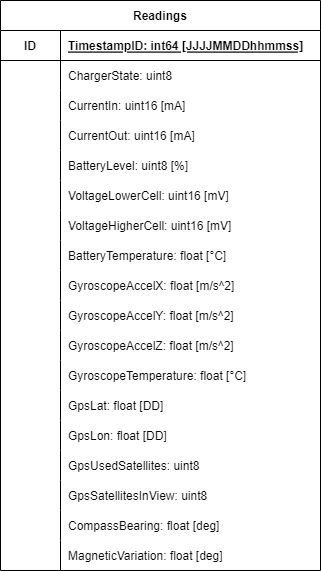
\includegraphics[width=0.5\textwidth]{pics/datenbankmodell.png}
    \caption{Datenbankmodell}
    \label{fig. Datenbankmodell}
\end{figure}
